\section{Validation experiments}\label{validationExperiments}

In addition to the experiments presented in Sections \ref{referenceResults} to \ref{additionalExperiments}, we present a new series of experiments in this section with the aim of validating particular properties of a system. These correspond firstly to experiments to validate correct operation under heavy concurrency. Secondly, we test whether the particular interface employed to execute queries on a system has some effect on performance or reliability.

\subsection{Concurrent execution with 32 streams}\label{concurrent32streams}

We test the ability of the systems to handle a high level of concurrency by running the TPC-DS Throughput Test with 32 streams, which adds up to 3,168 queries. Given the large number of total and concurrent queries, we employ the 10 GB scale factor, whereas, as noted earlier, our previous experiments employ the 1 TB scale factor.

We present in Figure \ref{fig:validationExperimentsStreams32TputTest} the result of this experiment. Databricks completes the test almost exactly 5 times faster. It is necessary to point out that in this case EMR Presto used a database in Parquet. Aiming for an accurate comparison, we can take the 34.67 hour time for EMR Presto using Parquet for the 1 TB 4 stream test in Section \ref{additionalExperimentsParquetVsORCPresto} and its analogous time of 6.85 hours of our reference results, Databricks turns out to be again almost exactly 5 times faster.

\begin{figure}
   \begin{center}
   \scalebox{0.65}{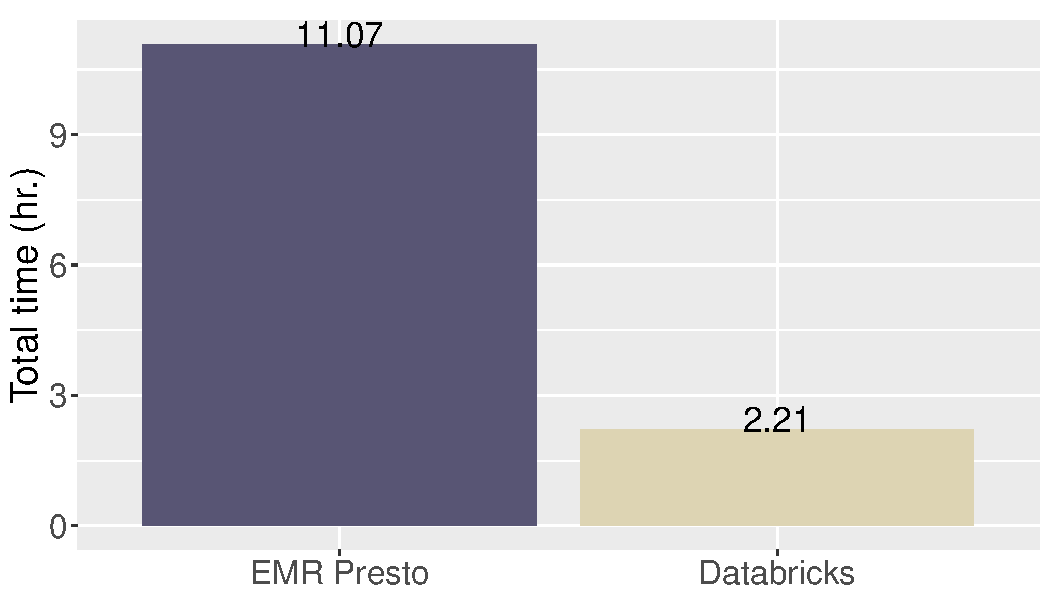
\includegraphics[width=7.0in]{imgs/validationExperiments/streams32/tput_totalHrTimeBarChart.pdf}}
   \end{center}
   \caption{EMR Presto vs. Databricks 32-stream 10 GB scale factor Throughput Test.}
   \label{fig:validationExperimentsStreams32TputTest}
\end{figure}

We can establish then that a much higher level of concurrency, 32 instead of 4 queries, did not fundamentally change the relative efficiency of both systems to deal with concurrency with respect to one another. It is also important to point out that no queries failed for either system, showing that both are capable of correctly scheduling them whilst appropriately allocating the available resources.

The relative efficiency of the two systems certainly can change if we move from the full TPC-DS Benchmark into a more specialized workload. In particular, it is interesting to consider a workload consisting of a high number of fast queries. In this case, no single query should hold resources for a long time. We defined such a workload by selecting 21 queries from TPC-DS and running a Throughput Test with 32 streams using them. Concretely, the queries are 3, 7, 8, 19, 27, 34, 42, 43, 46, 52, 53, 55, 59, 63, 65, 68, 73, 79, 82, 89, and 98.

The results can be seen in Figure \ref{fig:validationExperimentsImpalaKitTputTest}. EMR Presto now takes about double the time to complete this variant of the Throughput Test. Although the difference is significantly reduced, it still favors Databricks by a large margin. This difference cannot be attributed to an outlier query (or query instance) that turned out to be excessively slow among the query set. For Databricks completion times ranged from 5.9 seconds to 64.4 seconds, while for EMR Presto the range is from 3.3 seconds to 97.4 seconds.

\begin{figure}
   \begin{center}
   \scalebox{0.65}{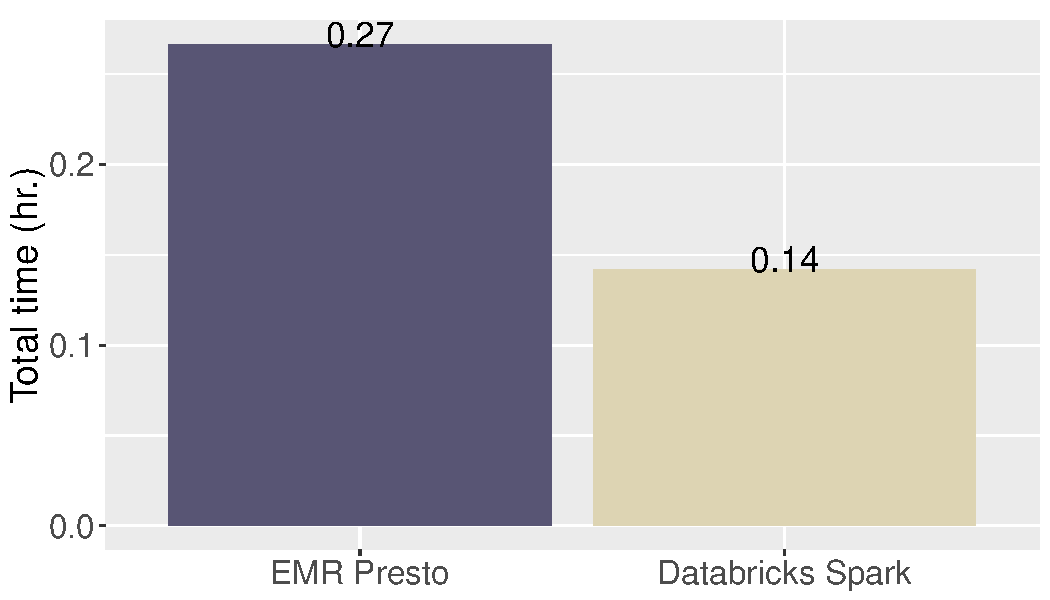
\includegraphics[width=7.0in]{imgs/validationExperiments/impalakit/tput_totalHrTimeBarChartReference.pdf}}
   \end{center}
   \caption{EMR Presto vs. Databricks 32-stream 10 GB scale factor Throughput Test selected queries.}
   \label{fig:validationExperimentsImpalaKitTputTest}
\end{figure}

\subsection{EMR Presto using JDBC vs. the CLI}\label{prestoJDBvsCLI}

Besides the JDBC interface supported by its associated driver, EMR Presto offers a command line interface (CLI) based on REST that also enables to submit queries and retrieve their results. We tested how the JDBC interface used in our reference results compares to the CLI in terms of performance and reliability.

For this purpose, we executed the 32-stream Throughput Test at the 10 GB scale factor with the CLI. Running this test resulted in a high number of failures, which traced back to the establishment of connections with the Presto server. These errors diminished when using 16 streams but only disappeared when restricting the test to 12 streams. This can be explained by the fact that when we use JDBC, we establish a single connection for each query stream, which runs as a separate thread. On the other hand, invoking the CLI requires issuing calls that translate to HTTP requests, in this case a new connection needs to be established for each query.

We believe that the need to establish new connections creates an overhead that is the main factor in reducing the efficiency of EMR Presto by around 20\%, as we can see in Figure \ref{fig:validationExperimentsPrestoCLITputTest}. This makes JDBC the preferred method to interact with EMR Presto.

\begin{figure}
   \begin{center}
   \scalebox{0.65}{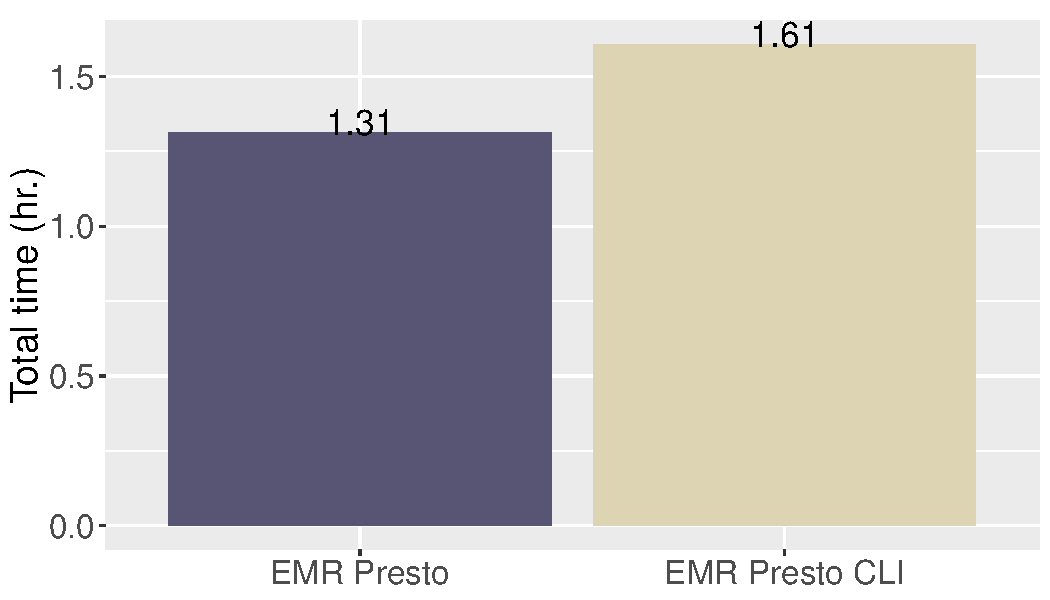
\includegraphics[width=7.0in]{imgs/validationExperiments/12streamsprestoResultsGraphs/tput_totalHrTimeBarChart.pdf}}
   \end{center}
   \caption{EMR Presto, JDBC vs. CLI, 12-stream 10 GB scale factor Throughput Test.}
   \label{fig:validationExperimentsPrestoCLITputTest}
\end{figure}

\subsection{Databricks JDBC interface with Simba driver}\label{databricksJDBC}

For the reference results, we executed SQL statements and queries via the SparkSession object, which is the single entry point for Spark in a programming environment. However, Databricks also offers a JDBC interface through a Spark Thrift Server, by means of a driver developed by Simba. The objective of the experiments in this subsection is to determine whether the JDBC interface offers comparable efficiency and reliability for Databricks users.

We can see from the results in Figure \ref{fig:validationExperimentsDatabricksJDBCPowerTest} and Figure \ref{fig:validationExperimentsDatabricksJDBCTputTest}, covering the 1 TB Power Test and Throughput Test, respectively, that no noticeable difference arises in performance. All the queries completed successfully as well. Importantly, the JDBC driver should be configured by including in the url the parameter UseNativeQuery=1. Otherwise, many queries fail due to SQL syntax incompatibility. Thus, JDBC is an efficient and reliable alternative to build applications that rely on Databricks.

\begin{figure}
   \begin{center}
   \scalebox{0.65}{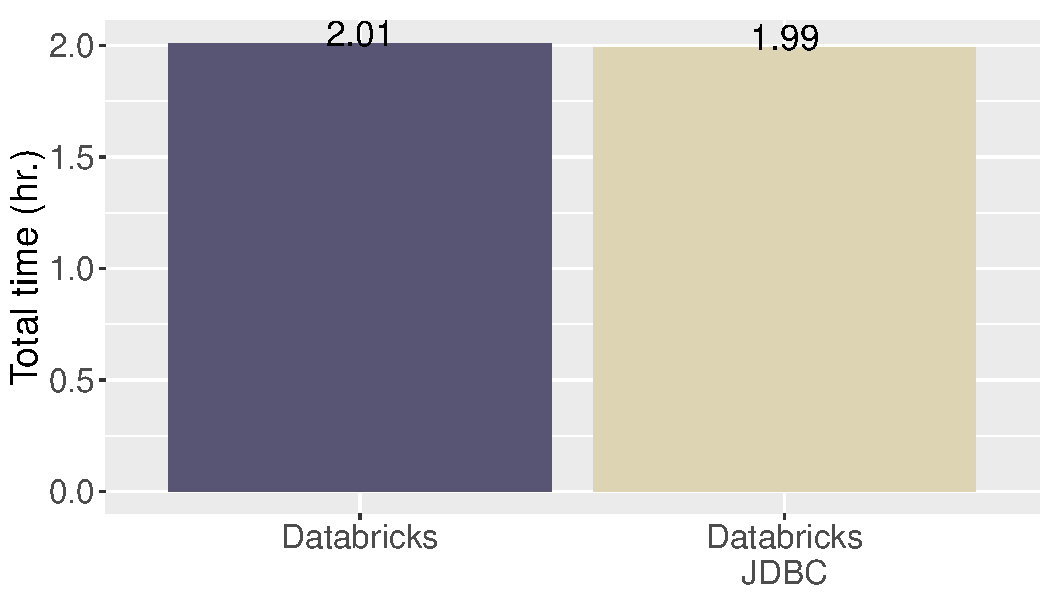
\includegraphics[width=7.0in]{imgs/validationExperiments/databricksjdbcResultsGraphs/power_totalHrTimeBarChart.pdf}}
   \end{center}
   \caption{Databricks, Job vs. JDBC, Power Test total time.}
   \label{fig:validationExperimentsDatabricksJDBCPowerTest}
\end{figure}

\begin{figure}
   \begin{center}
   \scalebox{0.65}{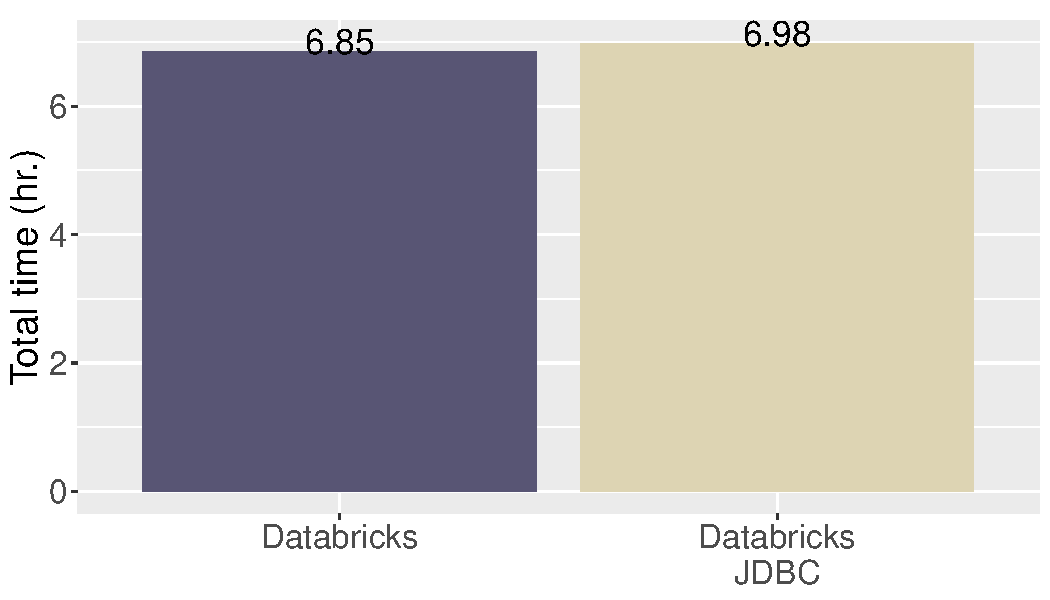
\includegraphics[width=7.0in]{imgs/validationExperiments/databricksjdbcResultsGraphs/tput_totalHrTimeBarChart.pdf}}
   \end{center}
   \caption{Databricks, Job vs. JDBC, Throughput Test total time.}
   \label{fig:validationExperimentsDatabricksJDBCTputTest}
\end{figure}

\subsection{Validation of previous results}

Since previous experiments by other parties have been carried out to evaluate the performance of EMR Presto and Databricks, it is of interest to look at their results, and, if possible, determining whether they are reasonably congruent with our own.

\subsubsection{Databricks Runtime 3.0 vs. EMR Presto}

The Databricks Engineering Blog published in July 2017 a performance study \cite{starburstReport} based on the TPC-DS Benchmark. We review their results covering Databricks and EMR Presto and compare them to our own. First, we state their hardware configuration alongside the one we adopt for this report in Table \ref{table:comparisonStudiesConfigurations}.

\begin{table}
  \centering
	\begin{tabular}{|l|l|l|l|l|l|}
	  \hline
		\textbf{Study} & \makecell[l]{\bf Number \\ \bf of nodes} & \makecell[l]{\bf EC2 \\ \bf instance \\ \bf types} & \textbf{vCPUs} & \textbf{Memory} & \textbf{Storage} \\ \hline
		\makecell[l]{Databricks \\ 2017} & 11 & r3.xlarge & 4 × 11 = 44 & \makecell[l]{30.5 × 11 = \\ 335.5 GB} & \makecell[l]{80 × 11 = \\ 880 GB \\ (EBS)} \\ \hline
		\makecell[l]{Present \\ report} & 8 & i3.2xlarge & 8 × 8 = 64 & \makecell[l]{61 × 8 = \\ 488 GB} & \makecell[l]{1900 × 8 = \\ 15200 GB \\ (SSD)} \\ \hline
	\end{tabular}
	\caption{Comparison of hardware configurations between studies.}
	\label{table:comparisonStudiesConfigurations}
\end{table}

In terms of number of CPU cores (independent of their type) and memory, the study in \cite{databricksReport} had at disposal about 70\% of the resources that we have in this report. The storage total capacity is far larger in our study, but since it is significantly under-utilized the main advantage it offers is speed, however, it is still not the dominant factor. We remark that an analysis of the configurations for Databricks and EMR Presto for both studies it out of the scope of our work.

\begin{figure}
   \begin{center}
   \scalebox{0.75}{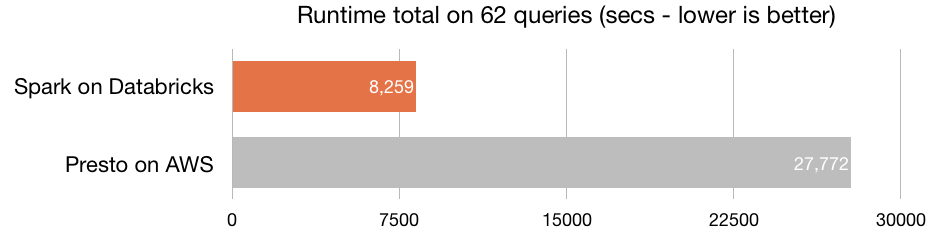
\includegraphics[width=7.0in]{imgs/validationExperiments/previousResults/databricksBlogGraph.png}}
   \end{center}
   \caption{Experimental results of Databricks Engineering Blog study.}
   \label{fig:validationExperimentsDatabricksBlogGraph}
\end{figure}

Figure \ref{fig:validationExperimentsDatabricksBlogGraph} shows the resulting total time obtained by the experiment in \cite{databricksReport} we focus on, which like our reference results used a 1 TB scale factor with the tables stored on S3. As it is pointed out in the figure, only 62 queries were evaluated in the experiment (as a Power Test), this is because the rest failed on EMR Presto. The total execution time for Databricks was about 2.3 hours, while it is about 7.7 for Presto, thus Databricks is about 3.3 times faster. Recalling our reference results presented in Section 4.2, which involve all 99 queries, the Databricks total time was about 2 hours in contrast to about 7.1 hours for EMR Presto, making Databricks around 3.6 times faster.

The proportions of the total execution times are very similar. Assessing the specific total execution times is complicated by the fact that the number of queries is different. However, given that the experiment in \cite{databricksReport} evaluated fewer queries but also had fewer hardware resources, these times seem congruent. Therefore, we do not find a major discrepancy between the two experiments.

\subsubsection{Starburst Presto Benchmarks}

Starburst offers several services based on Presto, notably cloud-computing clusters running Presto, either on AWS or Azure, and employing a proprietary cost-based optimizer (CBO) for queries. A white paper \cite{starburstReport} provides a description and benchmarking experiments.

Figure \ref{fig:validationExperimentsStarburstGraph1} and Figure \ref{fig:validationExperimentsStarburstGraph2} from \cite{starburstReport} present their results, again based on the TPC-DS Benchmark. It is noted as TPCH-DS in the figure most likely due to an error, with a second error being the key in Figure 83 that should use the key in Figure 82 instead\footnote{An excerpt of the white paper presented in https://www.starburstdata.com/technical-blog/starburst-presto-on-aws-18x-faster-than-emr/ does not show these errors.} . They provide results for 47 queries since the rest failed on the default Presto configuration. It is likely the 1 TB scale factor was used for these queries but that is not entirely clear from \cite{starburstReport}. The version of EMR Presto used in \cite{starburstReport} is 0.194, while we used 0.215.

\begin{figure}
   \begin{center}
   \scalebox{0.65}{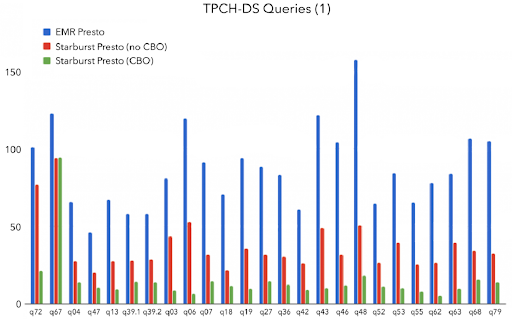
\includegraphics[width=7.0in]{imgs/validationExperiments/previousResults/starburstReport1.png}}
   \end{center}
   \caption{Starburst Presto experimental results (1).}
   \label{fig:validationExperimentsStarburstGraph1}
\end{figure}

\begin{figure}
   \begin{center}
   \scalebox{0.65}{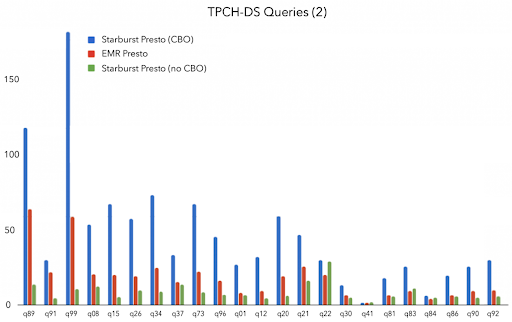
\includegraphics[width=7.0in]{imgs/validationExperiments/previousResults/starburstReport2.png}}
   \end{center}
   \caption{Starburst Presto experimental results (2).}
   \label{fig:validationExperimentsStarburstGraph2}
\end{figure}

The results clearly show significant timesavings when using Starburst Presto in comparison to EMR Presto. In almost all instances, its cost-based optimizer (CBO) can further reduce those execution times.

It is important to consider that the CBO requires column statistics for better results, whether we are speaking of the conventional Presto optimizer (that we assume available on EMR) or the optimizer offered by Starburst. In our experiments, we do not employ column statistics since the AWS Glue metastore does not support them.

These results raise the question of whether we would have obtained significantly better results if we used Starburst Presto instead of EMR Presto. A confident answer would require performing the actual experiments. We did compare the default Presto session configuration of the EMR Presto clusters we used with its analogous from a current Starbust Presto test cluster, and did not find, in our view, any major differences we had not addressed in our tuning efforts. Due to that reason, we are surprised of the large difference reported between Starburst Presto (without CBO) and EMR Presto. A concrete comparison of Starburst Presto with our current or new results for Databricks and EMR Presto is an alternative for future work.











